\documentclass{article}
\usepackage[polish]{babel}
\usepackage[utf8]{inputenc}
\usepackage{polski}
\frenchspacing
\setcounter{tocdepth}{2}
\usepackage{graphicx}
\graphicspath{ {images/} }

\begin{document}
	
\begin{titlepage}

\newcommand{\HRule}{\rule{\linewidth}{0.5mm}}

\center

%----------------------------------------------------------------------------------------

\textsc{\LARGE Politechnika Warszawska}\\[5mm]
\textsc{\LARGE Wydział Matematyki i Nauk Informacyjnych}\\[4cm]
 
%----------------------------------------------------------------------------------------

\textsc{\Huge Algorytmy Zaawansowane}\\[0.5cm]

%----------------------------------------------------------------------------------------

\HRule \\[0.4cm]
{ \LARGE \bfseries Wyznaczanie spójności krawędziowej grafu przez przepływ}\\[0.2cm]
 
%----------------------------------------------------------------------------------------

\HRule \\[0.4cm]
{  \bfseries Instrukcja użytkownika}\\[2.5cm]
 
%----------------------------------------------------------------------------------------

\begin{flushright}
\Large \emph{Autorzy:}\\[0.5cm]
Anna \textsc{Zawadzka}\\
Piotr \textsc{Waszkiewicz}\\[3.5cm]
\end{flushright}
%----------------------------------------------------------------------------------------

\vfill
{\large \today}\\[3cm]

\end{titlepage}
	
\newpage

\section{Dostarczone pliki}

Użytkownik otrzymuje następujący zestaw plików:

\begin{itemize}
    \item EdgeConnectivity.exe - plik wykonywalny
    \item Examples - folder z przykładowymi grafami w plikach .txt
\end{itemize}


%----------------------------------------------------------------------------------------

\section{Instrukcja}

Aby rozpocząć pracę z programem należy uruchomić plik EdgeConnectivity.exe, po czym wyświetlone zostanie okno aplikacji:
 
\begin{figure}[h]
\centering
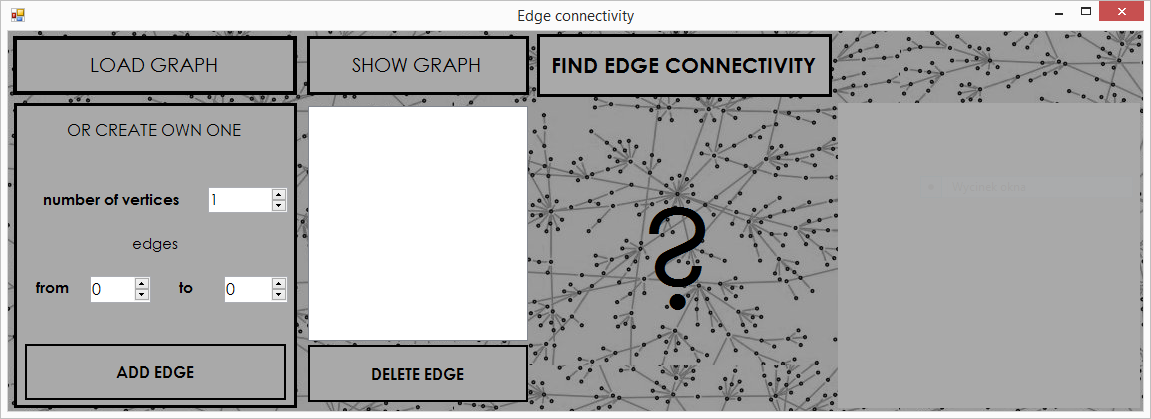
\includegraphics[scale=0.4]{01}
\caption{Okno aplikacj}
\end{figure}


Na tym etapie możliwe jest wczytanie grafu z pliku tekstowego. Należy użyć przycisku LOAD GRAPH, po czym otworzy się okno dialogowe do wyboru pliku. Program skonfigurowany jest w taki sposób, że początkowa lokalizacja wyboru pliku jest miejscem, w którym znajduje się plik EdgeConnectivity.exe. Plik wejściowy musi być w formacie .txt i mieć następującą strukturę:  pierwsza linia zawiera liczbę wierzchołków grafu $|V|$ oraz liczbę krawędzi $|E|$ oddzielone spacją, każda kolejna linia reprezentuje krawędź grafu zdefiniowaną przez numery wierzchołków, będących końcami krawędzi, oddzielone spacją. Kolejność podawania numerów wierzchołków w definicji krawędzi nie ma znaczenia, gdyż graf wejściowy jest nieskierowany. Zakładamy, że wierzchołki grafu numerowane są od 0.
Po wczytaniu pliku pojawi się lista krawędzi grafu, a w panelu do tworzenia i edycji grafu zmieni się liczba wierzchołków, na taką, jaka została podana w pliku wejściowym.
 
\begin{figure}[h]
\centering
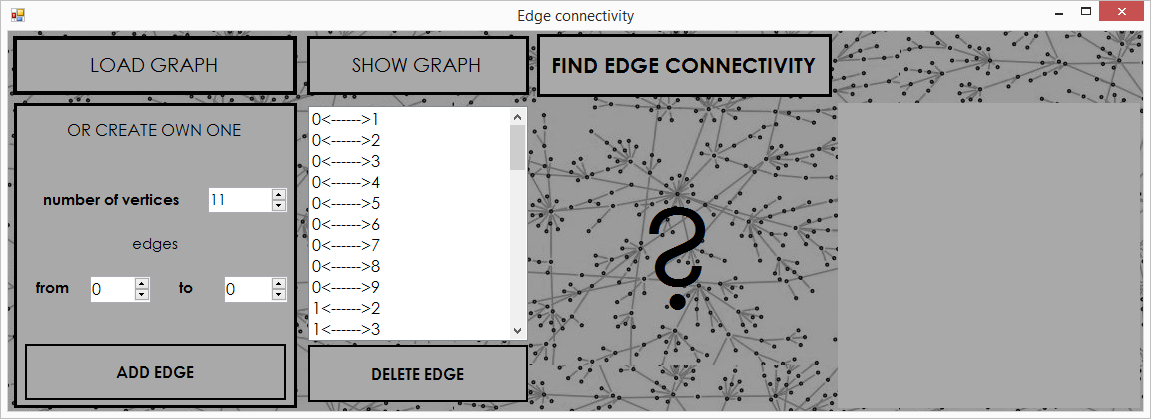
\includegraphics[scale=0.4]{02}
\caption{Okno aplikacj po wczytaniu grafu}
\end{figure}

Krawędzie, które znajdują się na liście można wybierać (klikając w odpowiednią) i usuwać za pomocą przycisku DELETE EDGE. Można również dodawać do grafu nowe krawędzie ustalając odpowiednie wartości numerów wierzchołków (from oraz to) i klikając w przycisk ADD EDGE. Numery wierzchołków zaczynają się od 0 i są nie większe niż ustalona liczba wierzchołków. Program gwarantuje, że jeśli w grafie istnieje krawędź o początku w wierzchołku u i końcu v, niemożliwe jest dodanie krawędzi o początku w wierzchołku v i końcu u (ponieważ w grafie nieskierowanym takie krawędzie traktowane są jako jedna), a także nie można dodać pętli, czyli krawędzi, której końcami jest ten sam wierzchołek.
Program umożliwia także utworzenie grafu od początku, należy ustalić liczbę wierzchołków oraz dodać odpowiednie krawędzie. Można modyfikować graf tak samo, jak w przypadku modyfikacji wczytanego grafu.
Przy zmianie liczby wierzchołków w programie, jeśli w pamięci istnieje graf, zostaje on usuwany i możliwe jest konstruowanie nowego grafu.
Program pozwala także na wizualizację grafu, należy użyć przycisku SHOW GRAPH, po czym w prawej części aplikacji pojawi się aktualny graf. Przy każdym użyciu przycisku SHOW GRAPH wizualizacja może się zmieniać, ponieważ za każdym razem rysowany jest nowy graf za pomocą algorytmu Fruchterman-Reingold.
 
\begin{figure}[h]
\centering
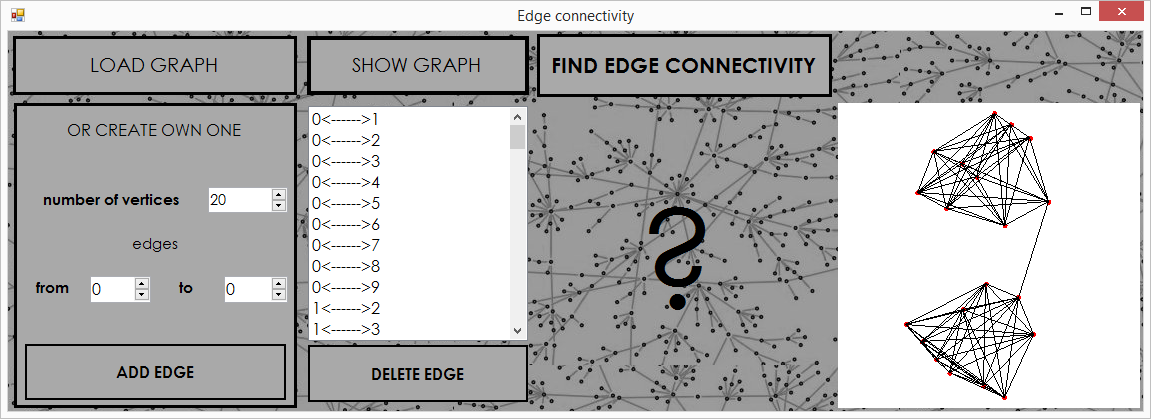
\includegraphics[scale=0.4]{03}
\caption{Okno aplikacj po wyświetleniu grafu}
\end{figure}
 
Jeżeli etap konstrukcji grafu jest już zakończony, można obliczyć jego spójność krawędziową. Należy użyć przycisku FIND EDGE CONNECTIVITY, po czym w miejsce znaku zapytania między listą krawędzi a oknem wizualizacji grafu pojawi się minimalna liczba krawędzi, które należy usunąć aby rozspójnić graf, czyli spójność krawędziowa.
 
\begin{figure}[h]
\centering
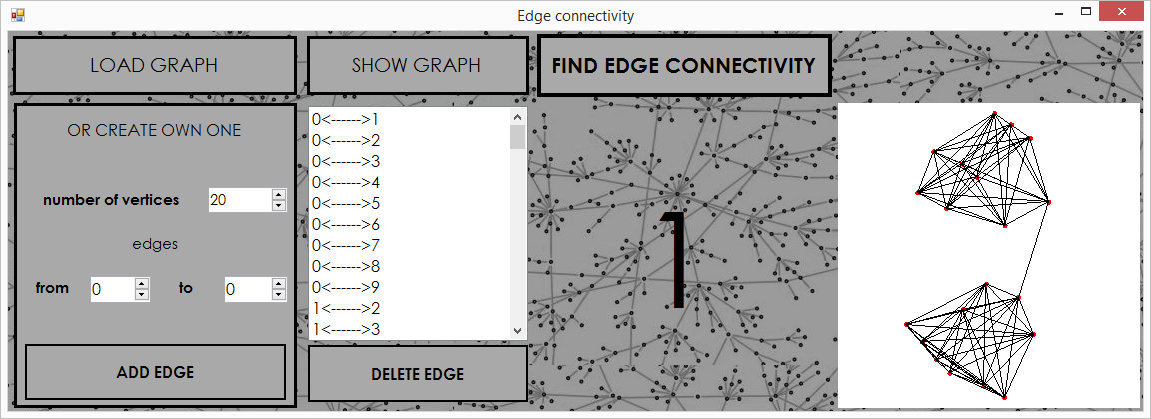
\includegraphics[scale=0.4]{04}
\caption{Okno aplikacj po znalezieniu spójności krawędziowej}
\end{figure}

W tym momencie można zakończyć pracę z programem, bądź wczytać lub utworzyć nowy graf.


\end{document}



